\subsection{UC-11 Visualizzazione del profilo personale da applicazione mobile}

\begin{figure}[H]
	\centering
	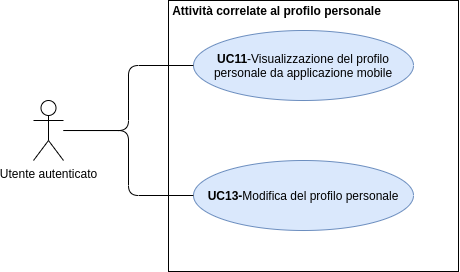
\includegraphics[width=\textwidth]{src/CasiDUso/immagini/ProfiloPersonale.png}
	\caption{UC-11,13.}
\end{figure}

\begin{itemize}
	\item \textbf{Attore primario:} utente autenticato;

	\item \textbf{Precondizioni:} l'utente è autenticato presso il sistema;

	\item \textbf{Postcondizioni:} l'utente visualizza i dati relativi al proprio profilo;

	\item \textbf{Scenario principale:}
		\begin{enumerate}
   			 \item  l'utente seleziona la sezione "il mio profilo";
    		 \item  il sistema elabora la richiesta e permette ora la visualizzazione dei seguenti dati:
   			\begin{itemize}
     			\item nome (UC-10.1);
         	    \item cognome (UC-10.2);
   			\end{itemize}
	   	\end{enumerate}
\end{itemize}


\begin{figure}[H]
	\centering
	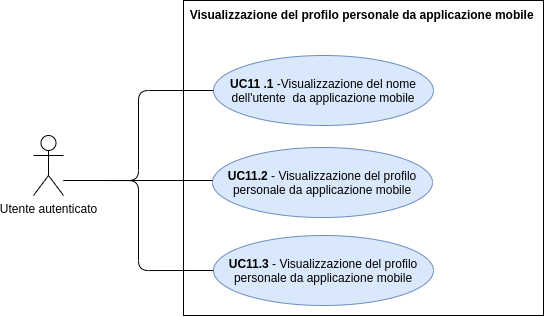
\includegraphics[width=\textwidth]{src/CasiDUso/immagini/SottocasiVisualizzazioneProfilo.png}
	\caption{Zoom-in visualizzazione profilo personale.}
\end{figure}

\subsubsection{UC-11.1 Visualizzazione del nome dell'utente da applicazione mobile}
\begin{itemize}
	\item \textbf{Attore primario:} utente autenticato;

	\item \textbf{Precondizioni:} l'utente è autenticato presso il sistema;

	\item \textbf{Postcondizioni:} l'utente visualizza il proprio nome sullo schermo;

	\item \textbf{Scenario principale:}
		\begin{enumerate}
    		\item  l'utente seleziona la sezione "il mio profilo";
    		\item  il sistema elabora la richiesta e permette ora la visualizzazione del nome dell'utente.
		\end{enumerate}
\end{itemize}

\subsubsection{UC-11.2 Visualizzazione del cognome dell'utente da applicazione mobile}
\begin{itemize}
	\item \textbf{Attore primario:} utente autenticato;

	\item \textbf{Precondizioni:} l'utente è autenticato presso il sistema;

	\item \textbf{Postcondizioni:} l'utente visualizza il proprio cognome sullo schermo;

	\item \textbf{Scenario principale:}
		\begin{enumerate}
    	\item  l'utente seleziona la sezione "il mio profilo";
    	\item  il sistema elabora la richiesta e permette ora la visualizzazione del cognome dell'utente.
		\end{enumerate}
\end{itemize}


\subsection{UC-12 Visualizzazione del profilo di un altro utente da applicazione web}

\begin{figure}[H]
	\centering
	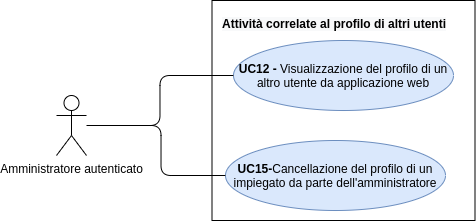
\includegraphics[width=\textwidth]{src/CasiDUso/immagini/AttivitaAdmin.png}
	\caption{UC-12,15.}
\end{figure}

\begin{itemize}
	\item \textbf{Attore primario:} amministratore autenticato;

	\item \textbf{Precondizioni:} l'amministratore è autenticato presso il sistema;

	\item \textbf{Postcondizioni:} l'amministratore visualizza i dati relativi al profilo del dipendente selezionato;

	\item \textbf{Scenario principale:}
	\begin{enumerate}
    	\item  l'amministratore seleziona la sezione con i profili degli utenti;
    	\item  il sistema elabora la richiesta e permette ora la visualizzazione dei seguenti dati:
    	\begin{itemize}
        	\item nome (UC-11.1 visualizzazione del nome dell'utente da applicazione web);
        	\item cognome (UC-11.2 visualizzazione del cognome dell'utente da applicazione web);
        	\item indirizzo e-mail (UC-11.3 visualizzazione dell'indirizzo e-mail dell'utente da applicazione web).
    	\end{itemize}
	\end{enumerate}
\end{itemize}

\begin{figure}[H]
	\centering
	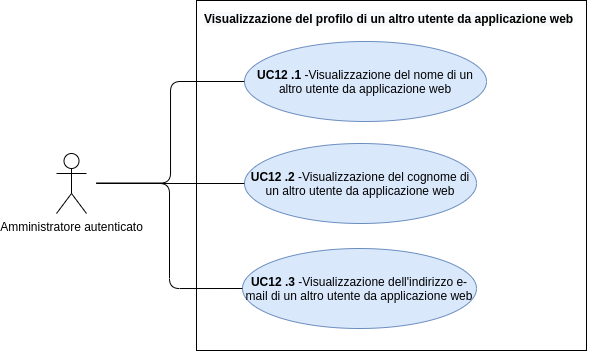
\includegraphics[width=\textwidth]{src/CasiDUso/immagini/SottocasiVisualizzazioneAdmin.png}
	\caption{Zoom-in visualizzazione profilo di un altro utente.}
\end{figure}

\subsubsection{UC-12.1 Visualizzazione del nome di un altro utente da applicazione web}
\begin{itemize}
	\item \textbf{Attore primario:} amministratore autenticato;

	\item \textbf{Precondizioni:} l'amministratore è autenticato presso il sistema;

	\item \textbf{Postcondizioni:} l'amministratore visualizza il nome dell'utente selezionato sullo schermo;

	\item \textbf{Scenario principale:}
	\begin{enumerate}
   		 \item  l'amministratore seleziona l'utente desiderato dalla sezione riepilogativa degli utenti registrati;
    	 \item  il sistema elabora la richiesta e permette ora la visualizzazione del nome dell'utente selezionato.
	\end{enumerate}
\end{itemize}

\subsubsection{UC-12.2 Visualizzazione del cognome di un altro utente da applicazione web}
\begin{itemize}
	\item \textbf{Attore primario:} amministratore autenticato;

	\item \textbf{Precondizioni:} l'amministratore è autenticato presso il sistema;

	\item \textbf{Postcondizioni:} l'amministratore visualizza il cognome dell'utente selezionato sullo schermo;

	\item \textbf{Scenario principale:}
		\begin{enumerate}
   			 \item  l'amministratore seleziona l'utente desiderato dalla sezione riepilogativa degli utenti registrati;
    		 \item  il sistema elabora la richiesta e permette ora la visualizzazione del cognome dell'utente selezionato.
		\end{enumerate}
\end{itemize}

\subsubsection{UC-12.3 Visualizzazione dell'indirizzo e-mail di un altro utente da applicazione web}
\begin{itemize}
	\item \textbf{Attore primario:} amministratore autenticato;

	\item \textbf{Precondizioni:} l'amministratore è autenticato presso il sistema;

	\item \textbf{Postcondizioni:} l'amministratore visualizza a video l'indirizzo e-mail dell'utente selezionato;

	\item \textbf{Scenario principale:}
		\begin{enumerate}
   			 \item  l'amministratore seleziona l'utente desiderato dalla sezione riepilogativa degli utenti registrati;
   			 \item  il sistema elabora la richiesta e permette ora la visualizzazione dell'indirizzo e-mail dell'utente selezionato.
		\end{enumerate}
\end{itemize}


